\let\lesson\undefined
\newcommand{\lesson}{\phantomlesson{Bài 4.}}


\setcounter{section}{2}
\section{Bài tập trắc nghiệm}
\begin{enumerate}[label=\bfseries Câu \arabic*:, leftmargin=1.7cm]
	\item \mkstar{1}\\
	Khi vật rắn tinh thể đang nóng chảy thì đại lượng nào của vật sau đây là không thay đổi?
	\begin{mcq}(4)
		\item Thể tích.
		\item Nội năng.
		\item Nhiệt độ.
		\item Hình dạng.
	\end{mcq}
\hideall{
\textbf{Đáp án C.}
}

\item \mkstar{1}\\
Điều nào sau đây là \textbf{sai} khi nói về nhiệt nóng chảy riêng?
\begin{mcq}
	\item Nhiệt nóng chảy riêng của chất rắn là nhiệt lượng cần cung cấp cho vật rắn trong quá trình nóng chảy.
	\item Đơn vị của nhiệt nóng chảy riêng là $\si{\joule/\kilogram}$.
	\item Các chất có khối lượng bằng nhau thì có nhiệt độ nóng chảy như nhau.
	\item Nhiệt nóng chảy riêng của chất rắn tỉ lệ thuận với khối lượng của vật.
\end{mcq}
\hideall{
\textbf{Đáp án C.}
}

\item \mkstar{1}\\
Điều nào sau đây là \textbf{đúng} khi nói về nhiệt nóng chảy riêng của chất rắn?
\begin{mcq}
	\item Nhiệt nóng chảy riêng của một chất rắn có độ lớn bằng nhiệt lượng cần cung cấp để làm nóng chảy $\SI{1}{\kilogram}$ chất đó ở nhiệt độ nóng chảy.
	\item Đơn vị của nhiệt nóng chảy riêng là joule trên kilogram $\left(\si{\joule/\kilogram}\right)$.
	\item Các chất khác nhau thì nhiệt nóng chảy riêng của chúng khác nhau.
	\item Cả A, B, C đều đúng.
\end{mcq}
\hideall{
\textbf{Đáp án D.}
}


\item \mkstar{1}\\
Nhiệt nóng chảy riêng của đồng là $\SI{1.8E5}{\joule/\kilogram}$. Câu nào dưới đây là \textbf{đúng}?
\begin{mcq}
	\item Khối đồng sẽ toả ra nhiệt lượng $\SI{1.8E5}{\joule}$ khi nóng chảy hoàn toàn.
	\item Mỗi kilogram đồng cần thu nhiệt lượng $\SI{1.8E5}{\joule}$ để hoá lỏng hoàn toàn ở nhiệt độ nóng chảy.
	\item Khối đồng cần nhu nhiệt lượng $\SI{1.8E5}{\joule}$ để hoá lỏng.
	\item Mỗi kilogram đồng toả ra nhiệt lượng $\SI{1.8E5}{\joule}$ khi hoá lỏng hoàn toàn.
\end{mcq}
\hideall{
\textbf{Đáp án B.}
}

\item \mkstar{1}\\
Đơn vị của nhiệt hoá hơi riêng của chất lỏng là
\begin{mcq}(4)
	\item $\si{\joule/\kilogram}$.
	\item $\si{\joule\cdot\kilogram}$.
	\item $\si{\kilogram/\joule}$.
	\item $\si{\joule}$.
\end{mcq}
\hideall{
\textbf{Đáp án A.}
}

\item \mkstar{1}\\
Nhiệt hoá hơi riêng của nước là $\SI{2.3E6}{\joule/\kilogram}$. Câu nào dưới đây là \textbf{đúng nhất}?
\begin{mcq}
	\item Mỗi lượng nước bất kì cần thu một lượng nhiệt $\SI{2.3E6}{\joule}$ để bay hơi hoàn toàn.
	\item Mỗi kilogram nước cần thu một lượng nhiệt là $\SI{2.3E6}{\joule}$ để bay hơi hoàn toàn.
	\item Mỗi kilogram nước sẽ toả ra một lượng nhiệt là $\SI{2.3E6}{\joule}$ khi bay hơi hoàn toàn ở nhiệt độ sôi.
	\item Mỗi kilogram nước cần thu một lượng nhiệt là $\SI{2.3E6}{\joule}$ để bay hơi hoàn toàn ở nhiệt độ sôi và áp suất chuẩn.
\end{mcq}
\hideall{
\textbf{Đáp án D.}
}

\item \mkstar{2}\\
Biết nhiệt nóng chảy riêng của nước đá là $\SI{3.34E5}{\joule/\kilogram}$. Nhiệt lượng cần cung cấp để làm nóng chảy $\SI{500}{\gram}$ nước đá ở $\SI{0}{\celsius}$ là
\begin{mcq}(4)
	\item $\SI{7E7}{\joule}$.
	\item $\SI{167}{\kilo\joule}$.
	\item $\SI{167}{\joule}$.
	\item $\SI{167e6}{\joule}$.
\end{mcq}
\hideall{
\textbf{Đáp án B.}\\
$$Q=m\lambda=\left(\SI{0.5}{\kilogram}\right)\cdot\left(\SI{3.34E5}{\joule/\kilogram}\right)=\SI{167}{\kilo\joule}.$$
}

\item \mkstar{2}\\
Biết nhiệt nóng chảy riêng của nước đá là $\SI{3.34E5}{\joule/\kilogram}$. Người ta cung cấp nhiệt lượng $\SI{5.01E5}{\joule}$ thì có thể làm nóng chảy hoàn toàn bao nhiêu kilogram nước đá?
\begin{mcq}(4)
	\item $\SI{16.7}{\kilogram}$.
	\item $\SI{1.5}{\kilogram}$.
	\item $\SI{8.35}{\kilogram}$.
	\item $\SI{0.668}{\kilogram}$.
\end{mcq}
\hideall{
\textbf{Đáp án B.}\\
$$m=\dfrac{Q}{\lambda}=\SI{1.5}{\kilogram}.$$
}

\item \mkstar{2}\\
Biết nhiệt dung riêng của nước là $c=\SI{4190}{\joule/\left(\kilogram\cdot\kelvin\right)}$ và nhiệt hoá hơi riêng của nước là $L=\SI{2.26E6}{\joule/\kilogram}$. Để làm cho $\SI{200}{\gram}$ nước ở $\SI{10}{\celsius}$ sôi ở $\SI{100}{\celsius}$ và $\SI{10}{\percent}$ lượng nước này hoá hơi khi sôi thì cần cung cấp một nhiệt lượng \textbf{gần nhất} là
\begin{mcq}(4)
	\item $\SI{169}{\kilo\joule}$.
	\item $\SI{121}{\kilo\joule}$.
	\item $\SI{189}{\kilo\joule}$.
	\item $\SI{212}{\kilo\joule}$.
\end{mcq}
\hideall{
\textbf{Đáp án B.}\\
Nhiệt lượng cần cung cấp:
$$Q=mc\left(100-t\right)+\SI{10}{\percent}mL\approx\SI{121}{\kilo\joule}.$$
}

\item \mkstar{3}\\
Cho biết nhiệt dung riêng của nước $\SI{4180}{\joule/\left(\kilogram\cdot\kelvin\right)}$ và nhiệt hoá hơi riêng của nước là $\SI{2.3E6}{\joule/\kilogram}$. Nhiệt lượng cần cung cấp cho $\SI{10}{\kilogram}$ nước ở $\SI{25}{\celsius}$ chuyển thành hơi ở $\SI{100}{\celsius}$ là
\begin{mcq}(4)
	\item $\SI{18450}{\kilo\joule}$.
	\item $\SI{26135}{\kilo\joule}$.
	\item $\SI{84500}{\kilo\joule}$.
	\item $\SI{804500}{\kilo\joule}$.
\end{mcq}
\hideall{
\textbf{Đáp án B.}\\
$$Q=mc\Delta t+mL=\SI{26135}{\kilo\joule}.$$
}

\item \mkstar{3}\\
Nước có nhiệt dung riêng $c=\SI{4180}{\joule/\left(\kilogram\cdot\kelvin\right)}$ và nhiệt hoá hơi riêng $L=\SI{2.3E6}{\joule/\kilogram}$. Nhiệt lượng toả ra khi $\SI{4}{\kilogram}$ hơi nước ở $\SI{100}{\celsius}$ ngưng tụ thành nước ở $\SI{22}{\celsius}$ là 
\begin{mcq}(4)
	\item $\SI{11504160}{\joule}$.
	\item $\SI{12504160}{\joule}$.
	\item $\SI{10504160}{\joule}$.
	\item $\SI{13504160}{\joule}$.
	
\end{mcq}
\hideall{
\textbf{Đáp án C.}\\
Nhiệt lượng toả ra khi $\SI{4}{\kilogram}$ hơi nước ở $\SI{100}{\celsius}$ ngưng tụ thành nước ở $\SI{22}{\celsius}$ là 
$$Q=mL+mc\left(t_0-t\right)=\SI{10504160}{\joule}.$$
}

\item \mkstar{3}\\
Để xác định nhiệt hóa hơi riêng của nước, người ta làm thí nghiệm sau: đưa $\SI{10}{\gram}$ hơi nước ở nhiệt độ $\SI{100}{\celsius}$ vào một nhiệt lượng kế chứa $\SI{290}{\gram}$ nước ở $\SI{20}{\celsius}$. Nhiệt độ cuối của hệ là $\SI{40}{\celsius}$. Cho biết nhiệt dung của nhiệt lượng kế là  $\SI{46}{\joule/\kelvin}$, nhiệt dung riêng của nước là $\SI{4.18}{\joule/\left(\gram\cdot\kelvin\right)}$. Nhiệt hoá hơi riêng của nước là 
\begin{mcq}(4)
	\item $\SI{6900}{\joule/\gram}$.
	\item $\SI{2265.6}{\joule/\gram}$.
	\item $\SI{4600}{\joule/\gram}$.
	\item $\SI{3200}{\joule/\gram}$.
\end{mcq}
\hideall{
\textbf{Đáp án B.}\\
Khi hệ cân bằng nhiệt, tổng nhiệt lượng trao đổi trong hệ bằng 0:
$$-m_\text{hơi}L+m_\text{hơi}c\left(t_\text{cb}-t_\text{hơi}\right)+m_\text{nước}c\left(t_\text{cb}-t_\text{n}\right)=0\Rightarrow L=\SI{2265.6}{\joule/\gram}.$$
}

\item \mkstar{3}\\
Đổ $\SI{100}{\gram}$ nước ở $\SI{40}{\celsius}$ vào một khối nước đá lớn ở $\SI{0}{\celsius}$. Cho nhiệt nóng chảy riêng của nước đá là $\lambda=\SI{80}{cal/\gram\cdot\kelvin}$ và nhiệt dung riêng của nước đá là $c=\SI{1}{cal/\gram\cdot\kelvin}$. Khối lượng nước đá tan chảy là
\begin{mcq}(4)
	\item $\SI{200}{\gram}.$
	\item $\SI{50}{\gram}.$
	\item $\SI{25}{\gram}.$
	\item $\SI{100}{\gram}.$
\end{mcq}
\hideall{
\textbf{Đáp án B.}\\
Khối lượng nước đá tan:
$$m=\dfrac{m_nc_n\Delta t}{\lambda}=\SI{50}{\gram}.$$
}


\item \mkstar{3}\\
Một chậu đựng hỗn hợp nước và nước đá có khối lượng $\SI{10}{\kilogram}$. Chậu để trong phòng và người ta theo dõi nhiệt độ của hỗn hợp. Đồ thị biểu thị sự phụ thuộc nhiệt độ theo thời gian cho ở hình bên. Cho nhiệt dung riêng của nước là $c=\SI{4200}{\joule/\left(\kilogram\cdot\kelvin\right)}$ và nhiệt nóng chảy riêng của nước đá là $\lambda=\SI{3.4E5}{\joule/\kilogram}$. Bỏ qua sự trao đổi nhiệt với chậu. Khối lượng nước đá trong hỗn hợp ban đầu là
\begin{center}
	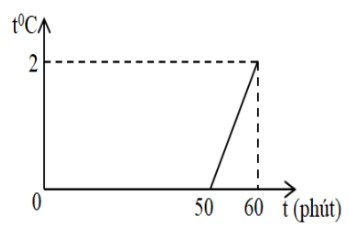
\includegraphics[width=0.4\linewidth]{../figs/VN12-Y24-PH-SYL-005P-1}
\end{center}
\begin{mcq}(4)
	\item $\SI{0.296}{\kilogram}$.
	\item $\SI{1.48}{\kilogram}$.
	\item $\SI{0.21}{\kilogram}$.
	\item $\SI{1.235}{\kilogram}$.
\end{mcq}
\hideall{
\textbf{Đáp án D.}\\
$$\dfrac{m_\text{đ}\lambda}{m_\text{hh}c\Delta t}=5\Rightarrow m_\text{đ}\approx\SI{1.235}{\kilogram}.$$
}

\item \mkstar{3}\\
Người ta thả một cục nước đá khối lượng $\SI{80}{\gram}$ ở $\SI{0}{\celsius}$ vào một cốc nhôm đựng $\SI{0.4}{\kilogram}$ nước ở $\SI{20}{\celsius}$ đặt trong nhiệt lượng kế. Biết khối lượng cốc nhôm là $\SI{0.2}{\kilogram}$. Cho nhiệt nóng chảy riêng của nước đá là $\SI{3.4E5}{\joule/\kilogram}$, nhiệt dung riêng của nhôm là $\SI{880}{\joule/\left(\kilogram\cdot\kelvin\right)}$ và của nước là $\SI{4180}{\joule/\left(\kilogram\cdot\kelvin\right)}$. Bỏ qua sự mất mát nhiệt do truyền ra ngoài. Nhiệt độ của nước khi nước đá đã tan hết là
\begin{mcq}(4)
	\item $\SI{4.5}{\celsius}$.
	\item $\SI{5.5}{\celsius}$.
	\item $\SI{6.5}{\celsius}$.
	\item $\SI{7.5}{\celsius}$.
\end{mcq}
\hideall{
\textbf{Đáp án A.}\\
Khi cân bằng nhiệt, tổng nhiệt lượng trao đổi trong hệ bằng 0:
$$m_\text{đ}\lambda+m_\text{đ}c\left(t_\text{cb}-0\right)+m_\text{n}c\left(t_\text{cb}-t_\text{n}\right)=0\Rightarrow t_\text{cb}\approx\SI{4.47}{\celsius}.$$
}

\item \mkstar{3}\\
Một viên đạn chì phải có tốc độ tối thiểu bằng bao nhiêu để khi nó va chạm vào vật cứng thì nóng chảy hoàn toàn? Cho rằng, $\SI{80}{\percent}$ động năng của viên đạn chuyển thành nội năng của nó khi va chạm; nhiệt độ của viên đạn trước khi va chạm là $\SI{127}{\celsius}$. Cho biết nhiệt dung riêng của chì là $\SI{130}{\joule/\left(\kilogram\cdot\kelvin\right)}$; nhiệt độ nóng chảy của chì là $\SI{327}{\celsius}$ và nhiệt nóng chảy riêng của chì là $\lambda=\SI{25}{\kilo\joule/\kilogram}$.
\begin{mcq}(4)
	\item $\SI{357}{\meter/\second}.$
	\item $\SI{324}{\meter/\second}.$
	\item $\SI{352}{\meter/\second}.$
	\item $\SI{457}{\meter/\second}.$
\end{mcq}
\hideall{
\textbf{Đáp án A.}\\
Nhiệt lượng cần thiết để viên đạn tăng nhiệt độ từ $\SI{127}{\celsius}$ lên $\SI{327}{\celsius}$ và nóng chảy hoàn toàn:
$$Q=mc\left(t-t_0\right)+m\lambda=51000m.$$
Áp dụng định lý động năng:
$$0-\dfrac{1}{2}mv^2_0=-\dfrac{Q}{0.8}$$
$$\Leftrightarrow \dfrac{1}{2}mv^2_0=\dfrac{51000m}{0.8}\Rightarrow v_0\approx\SI{357}{\meter/\second}.$$
}
\end{enumerate}
\section{Trắc nghiệm đúng/sai}
\begin{enumerate}[label=\bfseries Câu \arabic*:, leftmargin=1.7cm]
	\item \mkstar{2}\\
	Bảng dưới đây là nhiệt độ nóng chảy của một số chất.
	\begin{center}
		\begin{tabular}{|C{3cm}|C{1.25cm}|C{1.25cm}|C{1.25cm}|C{1.25cm}|C{1.25cm}|C{1.25cm}|C{1.25cm}|}
			\hline
			\thead{Chất} & Nhôm & Nước đá & Rượu & Sắt & Đồng & Thuỷ ngân & Muối ăn\\
			\hline
			\thead{Nhiệt độ nóng chảy\\ $\left(\si{\celsius}\right)$}& 660 & 0 & -117 & 1535 & 1083 & -39 & 801\\
			\hline
		\end{tabular}
	\end{center}
\begin{enumerate}[label=\alph*)]
	\item Chất có nhiệt độ nóng chảy cao nhất là đồng.
	\item Chất có nhiệt độ nóng chảy thấp nhất là thuỷ ngân.
	\item Có thể dùng nhiệt kế rượu để đo nhiệt độ thấp tới $\SI{-50}{\celsius}$.
	\item Có thể dùng nhiệt kế thuỷ ngân để đo nhiệt độ thấp tới $\SI{-50}{\celsius}$.
\end{enumerate}
\hideall{
\begin{enumerate}[label=\alph*)]
	\item Đúng.
	\item Sai. Chất có nhiệt độ nóng chảy thấp nhất là rượu.
	\item Đúng.
	\item Sai. Thuỷ ngân đã đông đặc ở $\SI{-39}{\celsius}$.
\end{enumerate}
}
\end{enumerate}
\section{Bài tập tự luận}
\begin{enumerate}[label=\bfseries Câu \arabic*:, leftmargin=1.7cm]
	\item\mkstar{2}\\
	Trên hình vẽ dưới đây biểu diễn đồ thị nhiệt độ của một chất theo thời gian trong quá trình đông đặc. Dựa vào đồ thị, em hãy trả lời các câu hỏi sau:
	\begin{center}
		\begin{tikzpicture}  
			\begin{axis}[  ultra thick,
				xmin=0,  
				xmax=28,  
				xtick={0,5,...,25},
				ytick={-40,-30,...,30},
				minor x tick num=1,
				minor y tick num=4,
				ymin=-48,  
				ymax=35, 
				samples=300,
				axis lines=center, 
				grid style={step=1, line width =0.4pt, color=gray!30!white},
				grid=both,
				major grid style={line width=0.8pt,gray!60!white},
				xlabel=$\xsi{t}{\left(\si{\text{phút}}\right)}$, 		ylabel=$\xsi{t}{\celsius}$,
				every axis y label/.style={at=(current axis.above origin),anchor=south},  
				every axis x label/.style={at=(current axis.right of origin),anchor=west},  ]
				\draw [ultra thick, red] (axis cs: 0,12) --(axis cs: 7.5,-40)--(axis cs: 25,-40)--(axis cs: 25.72,-45); 
				\filldraw[black] (axis cs:0,12) circle (1pt) node[right] {A};
				\filldraw[black] (axis cs:7.5,-40) circle (1pt) node[below] {B}; 
				\filldraw[black] (axis cs:25,-40) circle (1pt) node[below left] {C}; 
			\end{axis}
		\node[left] at (-0.1,3.2) {0};  
		\end{tikzpicture}
		
	\end{center}
\begin{enumerate}[label=\alph*)]
	\item Các đoạn AB và BC biểu diễn quá trình gì?
	\item Nhiệt độ ban đầu của chất này là bao nhiêu?
	\item Nhiệt độ đông đặc của chất này là bao nhiêu?
	\item Quá trình làm nguội và đông đặc diễn ra bao lâu?
\end{enumerate}
\hideall{
\begin{enumerate}[label=\alph*)]
	\item AB là quá trình chất này giảm nhiệt độ (quá trình làm nguội), BC là quá trình chất này đông đặc.
	\item Nhiệt độ ban đầu của chất này là $\SI{12}{\celsius}$.
	\item Nhiệt độ đông đặc của chất này là $\SI{-40}{\celsius}$.
	\item Qúa trình làm nguội diễn ra trong $\SI{7.5}{\text{phút}}$, quá trình đông đặc diễn ra trong $\SI{17.5}{\text{phút}}$.
\end{enumerate}
}
	\item \mkstar{3}\\
	Vận động viên chạy Marathon mất rất nhiều nước trong khi thi đấu. Các vận động viên thường chỉ có thể chuyển hoá khoảng $\SI{20}{\percent}$ năng lượng hoá học dự trữ trong cơ thể thành năng lượng dùng cho các hoạt động của cơ thể, đặc biệt là hoạt động chạy. Phần năng lượng còn lại chuyển thành nhiệt thải ra ngoài nhờ sự bay hơi của nước qua hô hấp và da để giữ nhiệt độ cơ thể ổn định. Nếu vận động viên dùng hết $\SI{11000}{\kilo\joule}$ trong cuộc thi thì có khoảng bao nhiêu lít nước đã thoát ra khỏi cơ thể? Coi nhiệt độ cơ thể của vận động viên hoàn toàn không đổi và nhiệt hoá hơi riêng của nước trong cơ thể vận động viên là $\SI{2.45E6}{\joule/\kilogram}$.
	\hideall{
	Lượng hơi nước thoát ra khỏi cơ thể vận động viên:
	$$m=\dfrac{\SI{80}{\percent}\cdot W}{L}\approx\SI{3.59}{\kilogram}.$$
}
\hideall{
\textbf{Đáp án D.}
}

\item \mkstar{3}\\
Để hàn các linh kiện bị đứt trong mạch điện tử, người thợ sửa chữa thường sử dụng mỏ hàn điện để làm nóng chảy dây thiếc hàn. Biết rằng loại thiếc hàn sử dụng là hỗn hợp của thiếc và chì với tỉ lệ khối lượng $63:37$, khối lượng một cuộn dây thiếc hàn là $\SI{50}{\gram}$. Biết thiếc và chì có nhiệt nóng chảy riêng lần lượt là $\SI{0.61E5}{\joule/\kilogram}$ và $\SI{0.25E5}{\joule/\kilogram}$. Nhiệt lượng mỏ hàn cần cung cấp để làm nóng chảy hết một cuộn dây thiếc hàn ở nhiệt độ nóng chảy bằng bao nhiêu?
\hideall{
$$\dfrac{m_t}{m_c}=\dfrac{63}{37}\xrightarrow{m_t+m_c=\SI{50}{\gram}}\begin{cases}
	m_t=\SI{31.5}{\gram}\\
	m_c=\SI{18.5}{\gram}
\end{cases}.$$
Nhiệt lượng mỏ hàn cần cung cấp để làm nóng chảy hết một cuộn dây thiếc hàn ở nhiệt độ nóng chảy:
$$Q=m_t\lambda_t+m_c\lambda_c=\SI{2384}{\joule}.$$
}

\item\mkstar{3}\\
Một ấm đun nước có công suất $\SI{500}{\watt}$ chứa $\SI{300}{\gram}$ nước. Cho nhiệt hoá hơi riêng của nước là $\SI{2E6}{\joule/\kilogram}$. Sau khi đun nước trong ấm đến nhiệt độ sôi, người ta để ấm tiếp tục đun nước sôi trong 2 phút. Bỏ qua sự mất mát nhiệt. Khối lượng nước còn lại trong ấm bằng bao nhiêu?
\hideall{
Lượng nước hoá hơi:
$$m'=\dfrac{\calP t}{L}=\SI{0.03}{\kilogram}=\SI{30}{\gram}.$$
Lượng nước còn lại trong ấm là
$$m=M-m'=\SI{270}{\gram}.$$
}

\item \mkstar{3}\\
Người ta trộn $m_1=\SI{500}{\gram}$ nước đá với $m_2=\SI{500}{\gram}$ nước ở cùng nhiệt độ $t_1=\SI{0}{\celsius}$ vào một xô nước ở nhiệt độ $\SI{50}{\celsius}$. Khối lượng tổng cộng của chúng là $m=\SI{2}{\kilogram}$. Tính nhiệt độ của xô nước khi có cân bằng nhiệt. Cho nhiệt dung riêng của nước $c=\SI{4200}{\joule/\left(\kilogram\cdot\kelvin\right)}$, nhiệt nóng chảy riêng của nước đá $\lambda=\SI{3.4E5}{\joule/\kilogram}$. Bỏ qua khối lượng và sự thu nhiệt của xô.
\hideall{
Khi cân bằng nhiệt, tổng nhiệt lượng trao đổi trong hệ bằng 0:
$$m_1\lambda+\left(m_1+m_2\right)c\left(t_\text{cb}-0\right)+\left(m-m_1-m_2\right)c\left(t_\text{cb}-t_0\right)=0$$
$$\Leftrightarrow 0,5\cdot\SI{3.4E5}{}+1\cdot4200\cdot t_\text{cb}+1\cdot4200\left(t_\text{cb}-50\right)=0\Rightarrow t_\text{cb}\approx\SI{4.76}{\celsius}.$$
}

\item \mkstar{3}\\
Bỏ $\SI{20}{\gram}$ tuyết có lẫn nước ở $\SI{0}{\celsius}$ vào nhiệt lượng kế chứa $\SI{250}{\gram}$ nước ở $\SI{15}{\celsius}$. Khi cân bằng nhiệt, nhiệt độ của nhiệt lượng kế giảm $\SI{5}{\celsius}$. Hỏi khối lượng nước lẫn trong tuyết là bao nhiêu? Biết nhiệt nóng chảy riêng của nước đá là $\lambda=\SI{3.4E5}{\joule/\kilogram}$, nhiệt dung riêng của nước $c=\SI{4200}{\joule/\left(\kilogram\cdot\kelvin\right)}$. Bỏ qua nhiệt dung của nhiệt lượng kế.
\hideall{
Gọi $m_1$, $m_2$ lần lượt là khối lượng của nước và đá trong tuyết.\\
Ta có:
\begin{equation*}
	m_1+m_2=\SI{0.02}{\kilogram}
\end{equation*}
Khi cân bằng nhiệt, tổng nhiệt lượng trao đổi trong hệ bằng 0:
$$m_2\lambda+\left(m_1+m_2\right)c\left(t_\text{cb}-0\right)+m_\text{n}c\left(t_\text{cb}-t_\text{n}\right)=0$$
$$\Rightarrow m_2\approx\SI{0.013}{\kilogram}=\SI{13}{\gram}.$$
Như vậy, khối lượng nước lẫn trong tuyết là $m_1\approx\SI{7}{\gram}.$
}
\item \mkstar{4}\\
Trong ruột cục nước đá lớn ở $\SI{0}{\celsius}$ có một cái hốc với thể tích bằng $V=\SI{160}{\centi\meter^3}$. Người ta rót vào hốc đó $\SI{60}{\gram}$ ở nhiệt độ $\SI{75}{\celsius}$. Cho khối lượng riêng của nước $D_1=\SI{1}{\gram/\centi\meter^3}$ và của nước đá $D_2=\SI{0.9}{\gram/\centi\meter^3}$, nhiệt dung riêng của nước là $c=\SI{4200}{\joule/\left(\kilogram\cdot\kelvin\right)}$ và để làm nóng chảy hoàn toàn $\SI{1}{\kilogram}$ nước đá ở nhiệt độ nóng chảy cần cung cấp cho khối nước đá này một nhiệt lượng $\SI{3.36E5}{\joule}$. Hỏi khi nước nguội hẳnn thì thể tích hốc rỗng còn lại là bao nhiêu $\si{\centi\meter^3}$?
\hideall{
Nhiệt lượng do nước toả ra để giảm nhiệt độ từ $\SI{75}{\celsius}$ về $\SI{0}{\celsius}$:
$$Q_\text{toả}=m_\text{n}c\left(0-t_\text{n}\right)=\SI{18900}{\joule}.$$
Thể tích nước rót vào hốc:
$$V_n=\dfrac{m_n}{D_1}=\SI{60}{\centi\meter^3}.$$
Khối lượng nước đá tan:
$$m_\text{đá}=\dfrac{Q_\text{thu}}{\lambda}=\dfrac{Q_\text{toả}}{\lambda}=\SI{56.25}{\gram}.$$
Thể tích nước đá bị tan là
$$V_\text{đ}=\dfrac{m_\text{đ}}{D_2}=\SI{62.5}{\centi\meter^3}.$$
Thể tích nước tạo thành do đá tan:
$$V_1=\dfrac{m_\text{đ}}{D_1}=\SI{56.25}{\centi\meter^3}.$$
Thể tích phần rỗng còn lại:
$$V+V_\text{đ}-V_1-V_\text{n}=\SI{106.25}{\centi\meter^3}.$$
}



\end{enumerate}